%% BioMed_Central_Tex_Template_v1.06
%%                                      %
%  bmc_article.tex            ver: 1.06 %
%                                       %

%%IMPORTANT: do not delete the first line of this template

%%%%%%%%%%%%%%%%%%%%%%%%%%%%%%%%%%%%%%%%%
%%                                     %%
%%  LaTeX template for BioVis 2014  %%
%%      article submissions     %%
%%          adapted from BMC    %%
%%          <8 Jan 2014>              %%
%% Liz Marai (g.elisabeta.marai@gmail.com) %%
%%                                     %%
%%%%%%%%%%%%%%%%%%%%%%%%%%%%%%%%%%%%%%%%%


%%%%%%%%%%%%%%%%%%%%%%%%%%%%%%%%%%%%%%%%%%%%%%%%%%%%%%%%%%%%%%%%%%%%%
%%                                                                 %%
%%%%%%%%%%%%%%%%%%%%%%%%%%%%%%%%%%%%%%%%%%%%%%%%%%%%%%%%%%%%%%%%%%%%%

%%% additional documentclass options:
%  [doublespacing]
%  [linenumbers]   - put the line numbers on margins

%%% loading packages, author definitions

\documentclass[twocolumn]{bmcart}% uncomment this for twocolumn layout 



%%% Load packages
%\usepackage{amsthm,amsmath}
%\RequirePackage{natbib}
%\RequirePackage{hyperref}
\usepackage[utf8]{inputenc} %unicode support
%\usepackage[applemac]{inputenc} %applemac support if unicode package fails
%\usepackage[latin1]{inputenc} %UNIX support if unicode package fails
\usepackage{graphicx}
\usepackage{color}
\usepackage[textsize=small,colorinlistoftodos]{todonotes}
\usepackage{algorithm}
\usepackage{algorithmicx}
\usepackage{algpseudocode}
\usepackage{xspace}

%%%%%%%%%%%%%%%%%%%%%%%%%%%%%%%%%%%%%%%%%%%%%%%%%
%%                                             %%
%%  If you wish to display your graphics for   %%
%%  your own use using includegraphic or       %%
%%  includegraphics, then comment out the      %%
%%  following two lines of code.               %%
%%%%%%%%%%%%%%%%%%%%%%%%%%%%%%%%%%%%%%%%%%%%%%%%%


%\def\includegraphic{}
%\def\includegraphics{}



%%% Put your definitions there:
\startlocaldefs
\endlocaldefs


% Defines usefull commands.
\newcommand{\ie}{i.e.,~}
\newcommand{\eg}{e.g.,~}

\algrenewcommand\algorithmicrequire{\textbf{Input:}}
\algrenewcommand\algorithmicensure{\textbf{Output:}}
\algnewcommand\And{\textbf{and}\xspace}
\algnewcommand\Or{\textbf{or}\xspace}

%%% Begin ...
\begin{document}

%%% Start of article front matter
\begin{frontmatter}

\begin{fmbox}
\dochead{Research}

%%%%%%%%%%%%%%%%%%%%%%%%%%%%%%%%%%%%%%%%%%%%%%
%%                                          %%
%% Enter the title of your article here     %%
%%                                          %%
%%%%%%%%%%%%%%%%%%%%%%%%%%%%%%%%%%%%%%%%%%%%%%

\title{Interactive Exploration of Ligand Movements through Multiscale Temporal Tunnels}

%%%%%%%%%%%%%%%%%%%%%%%%%%%%%%%%%%%%%%%%%%%%%%
%%                                          %%
%% Do not enter the authors here for        %%
%%  a double-blind review. Otherwise        %%
%% specify information, if available,       %%
%% in the form:                             %%
%%   <key>={<id1>,<id2>}                    %%
%%   <key>=                                 %%
%% Comment or delete the keys which are     %%
%% not used. Repeat \author command as much %%
%% as required.                             %%
%%                                          %%
%%%%%%%%%%%%%%%%%%%%%%%%%%%%%%%%%%%%%%%%%%%%%%
\author[
   addressref={aff1},
   email={furmanova@mail.muni.cz}
]{\inits{KF}\fnm{Katar\'{i}na} \snm{Furmanov\'{a}}}
\author[
   addressref={aff1},                   % id's of addresses, e.g. {aff1,aff2}
   email={jaresova@mail.muni.cz}   % email address
]{\inits{MJ}\fnm{Miroslava} \snm{Jare\v{s}ov\'{a}}}
\author[
   addressref={aff1,aff2},                   % id's of addresses, e.g. {aff1,aff2}
   email={xbyska@fi.muni.cz}   % email address
]{\inits{JB}\fnm{Jan} \snm{By\v{s}ka}}
\author[
   addressref={aff1},                   % id's of addresses, e.g. {aff1,aff2}
   email={xjurc@fi.muni.cz}   % email address
]{\inits{AJ}\fnm{Adam} \snm{Jur\v{c}\'{i}k}}
\author[
   addressref={aff2},                   % id's of addresses, e.g. {aff1,aff2}
   email={julius.parulek@uib.no}   % email address
]{\inits{JP}\fnm{J\'{u}lius} \snm{Parulek}}
\author[
   addressref={aff2},                   % id's of addresses, e.g. {aff1,aff2}
   email={Helwig.Hauser@uib.no}   % email address
]{\inits{HH}\fnm{Helwig} \snm{Hauser}}
\author[
   addressref={aff1},                   % id's of addresses, e.g. {aff1,aff2}
   email={kozlikova@fi.muni.cz}   % email address
]{\inits{BK}\fnm{Barbora} \snm{Kozl\'{i}kov\'{a}}}

%%%%%%%%%%%%%%%%%%%%%%%%%%%%%%%%%%%%%%%%%%%%%%
%%                                          %%
%% Enter the authors' addresses here        %%
%%                                          %%
%% Repeat \address commands as much as      %%
%% required.                                %%
%%                                          %%
%%%%%%%%%%%%%%%%%%%%%%%%%%%%%%%%%%%%%%%%%%%%%%

\address[id=aff1]{%                           % unique id
  \orgname{Masaryk University}, % university, etc
  %\postcode{15260}                                % post or zip code
  \city{Brno},                              % city
  \cny{Czech Republic}                                    % country
}
\address[id=aff2]{%                           % unique id
  \orgname{University of Bergen}, % university, etc
%  \street{210 South Bouquet},                     %
  %\postcode{15260}                                % post or zip code
  %\city{Williamsburg},                              % city
  \cny{Norway}                                    % country
}

%%%%%%%%%%%%%%%%%%%%%%%%%%%%%%%%%%%%%%%%%%%%%%
%%                                          %%
%% Enter short notes here                   %%
%%                                          %%
%% Short notes will be after addresses      %%
%% on first page.                           %%
%%                                          %%
%%%%%%%%%%%%%%%%%%%%%%%%%%%%%%%%%%%%%%%%%%%%%%

\begin{artnotes}
%\note{Sample of title note}     % note to the article
%\note[id=n1]{Equal contributor} % note, connected to author
%\note[id=n2]{Equal contributor} % note, connected to author
%\note[id=n3]{Equal contributor} % note, connected to author
%\note[id=n4]{Project leader and equal contributor} % note, connected to author
\end{artnotes}

\end{fmbox}% comment this for two column layout

%%%%%%%%%%%%%%%%%%%%%%%%%%%%%%%%%%%%%%%%%%%%%%
%%                                          %%
%% The Abstract begins here                 %%
%%                                          %%
%% Please refer to the Instructions for     %%
%% authors on http://www.biomedcentral.com  %%
%% and include the section headings         %%
%% accordingly for your article type.       %%
%%                                          %%
%%%%%%%%%%%%%%%%%%%%%%%%%%%%%%%%%%%%%%%%%%%%%%

\begin{abstractbox}

\begin{abstract} % abstract, must be under 350 words
%\parttitle{First part title} %if any
%Text for this section.

\parttitle{Background} TODO BK 

\parttitle{Results} TODO BK 

\parttitle{Conclusions}  TODO BK


%\parttitle{Second part title} %if any
%Text for this section.
\end{abstract}

%%%%%%%%%%%%%%%%%%%%%%%%%%%%%%%%%%%%%%%%%%%%%%
%%                                          %%
%% The keywords begin here                  %%
%%                                          %%
%% Put each keyword in separate \kwd{}.     %%
%%                                          %%
%%%%%%%%%%%%%%%%%%%%%%%%%%%%%%%%%%%%%%%%%%%%%%

\begin{keyword}
\kwd{Molecular Sequence Analysis}
\kwd{Molecular Structural Biology}
\kwd{Computational Proteomics}
\end{keyword}

% MSC classifications codes, if any
%\begin{keyword}[class=AMS]
%\kwd[Primary ]{}
%\kwd{}
%\kwd[; secondary ]{}
%\end{keyword}

\end{abstractbox}
%
%\end{fmbox}% uncomment this for twcolumn layout

\end{frontmatter}

%%%%%%%%%%%%%%%%%%%%%%%%%%%%%%%%%%%%%%%%%%%%%%
%%                                          %%
%% The Main Body begins here                %%
%%                                          %%
%% Please refer to the instructions for     %%
%% authors on:                              %%
%% http://www.biomedcentral.com/info/authors%%
%% and include the section headings         %%
%% accordingly for your article type.       %%
%%                                          %%
%% See the Results and Discussion section   %%
%% for details on how to create sub-sections%%
%%                                          %%
%% use \cite{...} to cite references        %%
%%  \cite{koon} and                         %%
%%  \cite{oreg,khar,zvai,xjon,schn,pond}    %%
%%  \nocite{smith,marg,hunn,advi,koha,mouse}%%
%%                                          %%
%%%%%%%%%%%%%%%%%%%%%%%%%%%%%%%%%%%%%%%%%%%%%%

%%%%%%%%%%%%%%%%%%%%%%%%% start of article main body
% <put your article body there>

%%%%%%%%%%%%%%%%
%% Background %%
%%
\section*{Background}
TODO BK + JP (Intro + RW)

The study of reaction processes between different types of molecules has been an important research problem already for decades.
A proper understanding of the processes occurring when two or more molecules react helps in the design of new chemical matters, e.g., in drug design or protein engineering.
Here, the researchers aim to combine a protein with a given ligand in order to design a new drug or to change protein properties and their function.
In these particular cases the ligand has to be transported from the outer solvent to the protein active site where the chemical reaction between the ligand and the amino acids surrounding the active site takes place.
The consecutive reaction then changes the composition and properties of both molecules. 
In protein engineering, for example, the goal is to alter the protein properties so that the new protein is, e.g., more stable and resistant to organic cosolvents~\cite{Koudelakova2013}.

The design complexity of such reactions lies namely in the transportation of the ligand to the protein active site.
As the active site is usually buried deeply in the protein structure and thus inaccessible directly from its surface, the ligand has to find a suitable transportation path through the protein structure.
This process, called molecular docking, is very complex, lengthy, and its analysis is heavy on computational resources. 
Therefore, researchers aim at solutions that simplify and ease the analysis for proper ligand binding.
Currently available solutions often focus on detection of possible ligand transportation paths through the protein, called tunnels.
These solutions are mostly based on the geometric analysis, which lead to the tunnel detection in the end, e.g., CAVER~\cite{Chovancova2012}, MOLE~\cite{Sehnal2013}, or MolAxis~\cite{Yaffe2008}.
Other approaches, such as MoMA-LigPath~\cite{Devaurs}, aim at simulating the ligand transportation itself.
Nevertheless, simulating the ligand docking using current computational approaches is still a challenging problem.
There are several available variants of molecular simulation methods devised specifically to this problem. 
Among these Steered Molecular Dynamics~\cite{Isralewitz} and Random Acceleration Molecular Dynamics~\cite{Ludemann} are able to simulate the ligand binding. 
Such simulations produce a large amount of data containing the ligand movements that are to be explored by the domain expert.
As the length of these simulations reaches often hundreds of thousands of time steps, it becomes impossible for the domain experts to visualize and observe the ligand movement in a frame-by-frame manner.
Moreover, the simulation often contains movements that are irrelevant to the ligand binding.
For example, a significant portion of the simulation the ligand usually spends outside the protein searching for a proper tunnel gorge to enter the molecule. 
It also often happens that the ligand enters the molecule via a wrong tunnel and is then evicted from the molecule and searches for the entrance repeatedly.
Therefore, the "true" active site entering can be in fact captured in a smaller subset of the original sequence.

In this paper, we propose a new visual analysis system that addresses the aforementioned challenges, i.e.,  the transportation of a ligand to the active site. 
We aim to provide the domain experts with a tool for intuitive and interactive exploration of already captured molecular dynamics simulation containing the process of ligand binding. 
Using our proposed solution the users are able to distinguish between the parts of the simulation where the ligand searches for the proper path to the active site (searches the tunnel gorge or enters the wrong tunnel) and the part where the ligand finally leads to and reaches the active site.

{\color{red} CHANGE
Here, we introduce four dedicated methods for simplification of the original trajectory.
These methods can simplify the ligand path hierarchically, thus providing several levels of detail (LOD), which can be interactively examined.
In the most abstracted view, represented as the top-most LOD, the temporal tunnel shows only the significant shifts of the ligand towards the active site. 
Here, the user can interactively brush time intervals, which automatically reveals and adopts the temporal tunnel to the selected interval.
This abstracted representation, providing the brushing capabilities, is interactively linked with the 3D visualization where the 3D shape of the temporal tunnel for the given temporal window is displayed.
Further, our tool enables to explore the amino acids surrounding the ligand along its path to the active site as well.

Our proposed solution was thoroughly tested and evaluated by the domain experts from protein engineering.
They performed the evaluation on their own simulations and their feedback is described in....}

\section{Related Work}
The interactive exploration of ligand paths through protein structures is a complex problem that requires an elaborate analysis of existing and convenient approaches.
As our system addresses several areas, this section will be divided with respect to these areas as well. 
Studying the ligand transport path is tightly related to the analysis of its trajectory.
Thus, the first part will cover the topic related to the trajectory analysis, simplification, and visualization.
Then the existing representations of tunnels and their surrounding amino acids will be addressed.

\subsection{Trajectory Analysis, Simplification, and Visualization}
When searching for the most appropriate trajectory simplification method, the taxonomy of different movement patterns introduced by Dodge et al.~\cite{Dodge2008} can help to categorize the type of motion and to propose an appropriate solution for the analysis and simplification.
Then, Andrienko et al.~\cite{andrienko2013} describe a legacy of tools and approaches to analyze trajectory data.
With respect to the trajectory simplification, they introduce two approaches to data abstraction representing a necessary step to achieve the reduction of the data in order to achieve informative visualizations.
The first approach is characterized by omitting unnecessary positions and segments, while the second exploits data subsampling.
On the other hand, they state that there is no general method to sample trajectories.
Thus the suitability of particular sampling method is deduced from what information is considered important.
A recent work of Vrotsou et al.~\cite{Vrotsou2015} introduce a systematic stepwise methodology for trajectory simplification with emphasis on visual analysis.
Even though they primarily developed the tool to analyze three dimensional trajectories, it is not limited to them only.

In the field of molecular biology as well as systems biology, there are several examples of methods focusing on trajectory analysis.
Bidmon et al.~\cite{bidmon2008} present an abstract way of identification and visualization of solvent molecules' pathways within molecular dynamics. 
In comparison to previous solutions, their approach preserves valuable information on the directions and velocities of water molecules routing along these paths. 
Another approach that describes a guidance through a complex simulation trajectories in systems biology is presented by Luboschik et al.~\cite{Luboschik2012}. 
The method addresses biochemical reaction networks and aims to provide the users with a tool for investigating the overall behavior of a modeled system and detailed behavior at the same time.

\subsection{Visualization of Cavity and Tunnel Features}
Phillips et al.~\cite{phillips2010} propose a method to quantitatively estimate molecular features, e.g., volume and surface areas, via ray-casting technique. This involves computation of cavities.
Lindow et al.~\cite{LindowBH11} introduce a technique that allows to extract significant paths from the molecules. 
In their approach the authors utilize Voronoi diagram of spheres. 
Their final visualization is achieved by means of placing light sources on the extracted paths to enhance the presence of tunnels.
Parulek et al.~\cite{parulek2012} exploit scatterplots to communicate the evolution of protein voids. 
In their later study~\cite{parulek2013} they also suggest to utilize amino acids physico-chemical properties related to cavities to help users to navigate through their occurrences. 
The visualization is then achieved in the focus and context manner.
Lindow et al. \cite{Lindow2013} present an approach for visualization of temporal evolution of cavities in a temporal graph, which, to a certain extent, resembles our temporal tunnel model. 
In this work they focus on the interactive exploration of the dynamics of protein cavities that can form the transportation path for a ligand. 
They calculate and visualize the cavity volume and analyze the time-dependent changes of the cavity structure.
The cavity dynamics is captured by rendering the cavities in a single image. 
The final visualization is achieved through the molecular surface representation colored according to time. 
Krone et al.~\cite{krone2013features} present a similar approach, where they extract and track tunnels in MD simulations. They exploit temporal graphs to communicate the evolution of surface areas of tunnels. In our technique, we go one step further, where in addition, we incorporate the ligand-protein interaction information and provide users with the means to navigate through details of this interaction. Moreover, we analyze sequences of several thousands of frames, which is not the case in aforementioned approaches.
Kozlikova et al.~\cite{kozlikova2014vcbm} propose a way to seamlessly visualize the geometry and shape of tunnels across MD simulation. Here, they aim at 3D visualization solely, which is not suitable way of exploring and understanding of thousands of simulation time-steps.
Byska et al.~\cite{byska2016} introduce an approach to interactively explore the tunnel objects in MD simulations. Similarly to our approach they visualize the time-varying tunnel as a profile graph that includes information on surrounding amino acids. Nevertheless, they focus on a single tunnel instance and do not provide the means to explore the ligand-protein interaction.

%-------------------------------------------------------------------------
\section{Problem Description and Input Data}
When studying long molecular dynamics simulations, the researchers have to face namely the following high-level tasks:
\begin{itemize}
\item Detect the part of the simulation where the ligand enters the protein and finally reaches the active site.
\item Explore this route in detail and detect its bottlenecks.
\end{itemize}
In consequence, these steps are performed in order to reveal the parts of the trajectory where the ligand gets stuck.
It means that in such parts there are some obstacles made by the surrounding amino acids.
These obstacles can be geometric (the empty space between these amino acids is too narrow) or physico-chemical (the properties of the amino acids are incompatible with the ligand properties), or their combination.
The geometric obstacles can be detected by using an algorithm for tunnel computation in molecular dynamics (e.g., CAVER~\cite{Chovancova2012} or MOLE~\cite{Sehnal2013}).
These tools are able to produce the information about time evolution of individual tunnels and for each tunnel detect its bottleneck -- the narrowest part limiting the size of the ligand aiming to pass through this tunnel.
Figure~\ref{fig:tunnel} shows an example of small ligand passing through a tunnel computed by CAVER algorithm and visualized using CAVER Analyst~\cite{Kozlikova2014}. 
The tunnel is colored with respect to the hydrophobicity of the surrounding amino acids and the geometric bottleneck of the tunnel is clearly visible.

\begin{figure}[htb]
	\centering
  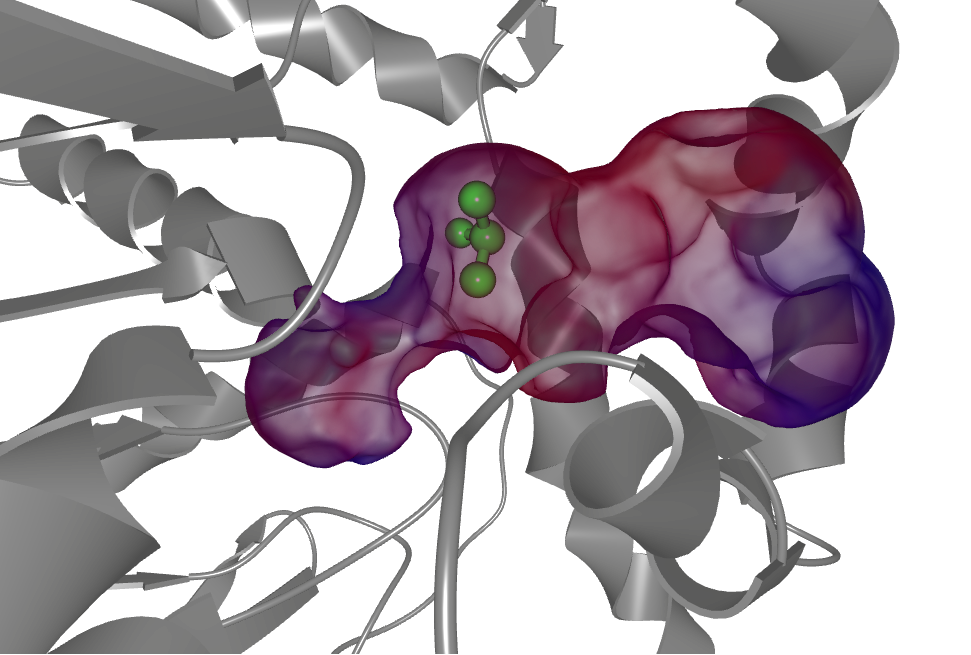
\includegraphics[width=1\linewidth]{img/tunnel.png}
  \caption{\label{fig:tunnel} Small ligand (green) passing through a tunnel represented by the transparent surface. The surface encloses the available empty space along the tunnel centerline and is colored with respect to the hydrophobicity of the surrounding amino acids (hydrophobic -- red, hydrophylic -- blue, neutral -- violet). The active site is located in the left ending of the tunnel.}
\end{figure}

However, this bottleneck can be to some extent influenced by the passing ligand and this influence is also determined by the physico-chemical properties of the ligand and the bottleneck-lining amino acids (e.g., hydrophobicity or partial charges of individual atoms).
To reveal such dependencies, it requires the involvement and experience of the domain expert who has to study the ligand trajectory captured in the molecular dynamics simulation.
And for such task a proper visual representation and guidance through such large data is substantial.

In protein engineering, all these effort can finally lead to the detection of amino acids along the ligand trajectory which caused problems, i.e., were the key players in situations when the ligand gets stuck.
Such amino acids are then the best candidates for subsequent mutation of the protein chain when these amino acids are replaced by more suitable ones wrt. their size and properties.
On the other hand, in drug design the aim is to propose modifications of the ligand to increase the binding likelihood in order to design a better drug produced from this ligand.

The input data is obtained from the simulations of molecular dynamics which contains the movements of the protein and one or more ligands.
Ligands can follow two main routes -- they can be transported from the outside environment to the protein active site or vice versa (after the desired reaction the product leaves the protein).

The length of the simulations may vary from few hundreds to hundreds of thousands of time steps.  
This depends namely on the ligand velocity and its ability to find the proper path to the active site.
Figure \ref{fig:lig_movement} shows an example of a ligand trajectory consisting of $50.000$ time steps. 

\begin{figure}[htb]
	\centering
  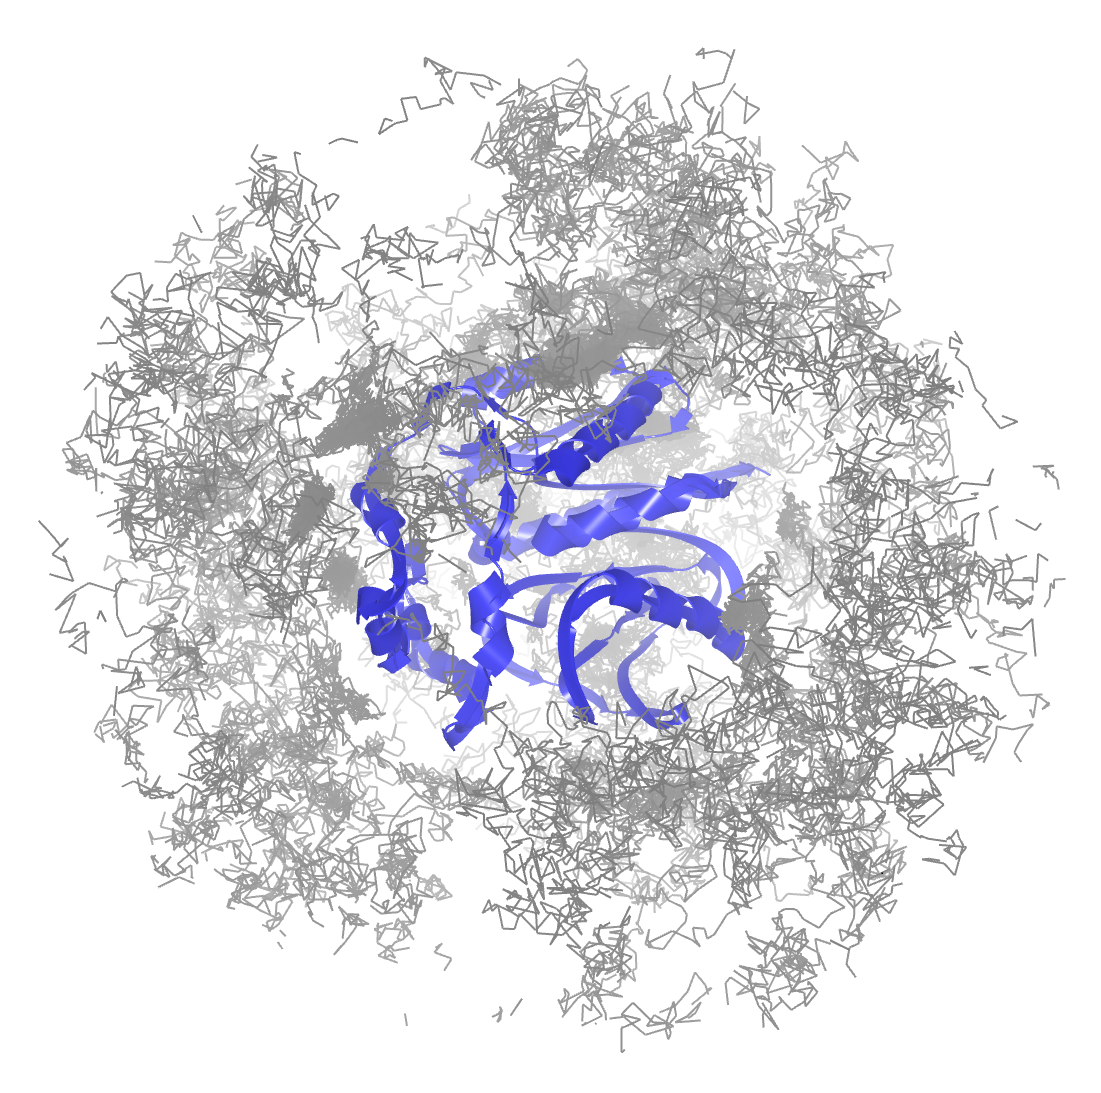
\includegraphics[width=0.95\linewidth]{img/lig_movement.png}
  \caption{\label{fig:lig_movement} Ligand trajectory (gray) for a simulation containing $50.000$ time steps.}
\end{figure}

Long simulations can often contain many time steps when the ligand followed an impasse -- it tried to find the proper entrance point to the protein (tunnel gorge) or entered a wrong tunnel and had to return.
Such parts of the simulation could be of less interest so that the user should be provided with a possibility to filter them out and focus only on the interesting parts.


\section*{Method}
\subsection*{Overview + workflow - BK}

\subsection*{Temporal Tunnel - JB}
\label{Sec:TemporalTunnel}
\todo{přehodil jsem sekci, sem, bo si myslím, že ji chceme použít aj v simplifikaci ne? + minimálně bude třeba o ní vědět při definování empy space atributu}

\todo{Nevím jak začít .... chce to asi nějakou motivaci proč vůbec temporal tunnel} 

We define the temporal tunnel as a set of spheres where the number of spheres corresponds to the number of time steps in the simulation.
Additionally, each sphere defines the maximum empty space surrounding the ligand, and as the consequence also contains the ligand, in the given time step {\color{red}(see Figure~\ref{XY})}.

In order to compute such temporal tunnel we can either utilize the pre-computed information about protein tunnels (\eg using CAVER~3.0) or approximate information about the empty space surrounding the ligand manually. 
The first method is more precise but computationally more expensive, while the second approach is faster but {\color{red}can be highly inaccurate} {\color{red}see Section~\ref{XYZ} for experimental comparison)}. 
Nevertheless, in both cases we need to determine a single sphere which will be part of temporal tunnel for each time step.

When using the pre--computed data we basically obtain a set of spheres defining the shape of the tunnel in each time step ({\color{red} see Section/Paper about CAVER}). 
Since we also have a ligand position \todo{někde bude třeba definovat ligand position} in each time step we can utilize the aforementioned information about protein tunnels to determine single tunnel sphere containing the ligand in the given time. 
The whole temporal tunnel then can be build simply by selecting the closest sphere to the ligand which is also wide enough \todo{wide enough není zprogramováné} to enclose fully it in each time step. \todo{ty poslední dvě věty se asi opakují.}

%The closest sphere can be find simply by measuring the distance between the center of mass of ligand and center of each sphere.  

{\color{red} Už nestíhám, ale ta druhá metoda byla popsána v předchozím článku, takže jí z tama můžeme vytáhnout - možná to ještě udělám později, zatím teda takto.}


\subsection*{Trajectory Simplification - AJ}
When visualizing the ligand trajectory in its original form, e.g., using a line strip of consecutive ligand positions, the visualization becomes very crowded even when analyzing only few hundreds of snapshots (see Figure~\ref{fig:crowded} left).
Therefore, it is necessary to simplify the original trajectory data and to visualize this simplified version.
In this manner, we enable the user to deduce the information about significant ligand movements directly from its 3D visualization.

\begin{figure}
	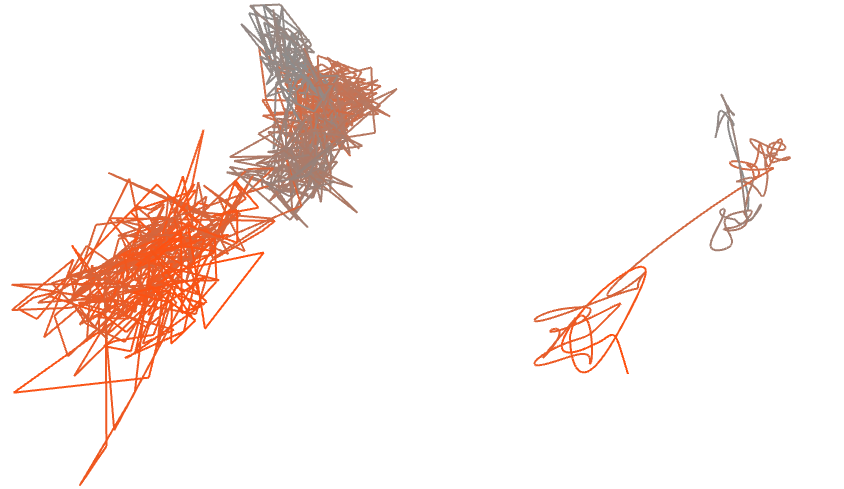
\includegraphics[width=0.95\linewidth]{img/crowded-combined.png}
\caption{Visualization of 800 snapshots of a ligand trajectory using line strip.
Visualization of the original trajectory is crowded (left).
On the other hand, visualization of the simplified trajectory clearly reveals its possible important parts (right).
The trajectory is colored by time from beginning (gray) towards its end (orange).}
\label{fig:crowded}
\end{figure}

We propose two types of ligand trajectory simplification: i) automatic and ii) interactive.
The automatic simplification is applied to the whole original trajectory, while the interactive one enables fine user-regulated control over the level of simplification of individual parts of the trajectory.
%In fact, the automatic simplification can be viewed as an iterative application of the manual simplification.
%, since its design was aligned with the workflow of a biochemist. - dala by som prec, postradam logicku navaznost
\subsubsection*{Interactive Simplification}

First, we will describe the algorithm for the interactive trajectory simplification (see Algorithm~\ref{alg:simplify}).
The input of the algorithm consist of trajectory $T_{in}$ and interval $I$ which denotes a part where the trajectory should be simplified.
%a data structure describing the simplification ($S$).
%More precisely, $S$ is a list of consecutive intervals that span the whole trajectory.
%Each interval in $S$ is assigned with a simplification level and as such describes amount of simplification of a respective part of $T_{in}$.
%This representation enables simplification of different parts of $T_{in}$ using different level of detail.
As a first step, the algorithm retrieves from a cache the current visualized trajectory $T'$ together with its simplification $S'$.
Structure $S'$ is a list of consecutive intervals that span the whole trajectory.
Each interval in $S'$ is assigned with a simplification level and as such describes the amount of simplification of a respective part of $T_{in}$.
This representation enables the simplification of different parts of $T_{in}$ using different levels of detail.
In the next step, the updated simplification $S$ is obtained by applying $I$ to $S'$.
Then, it is decided whether $T'$ can be incrementally updated to obtain $T_{out}$.
%If so, an interval $\Delta I$ which updates $S'$ to $S$ is obtained and the current visualized trajectory $T'$ is simplified on $\Delta I$ resulting in $T_{out}$.
This is true when the level of simplification of $T'$ at the updated interval $I$ is lower than the desired level of simplification.
In this case, the current visualized trajectory $T'$ is simplified on $I$ resulting in $T_{out}$.
%a difference of $S$ and $S'$ results in a single interval
Otherwise, the visualized trajectory $T'$ cannot be used and the simplified trajectory has to be computed from scratch using $T_{in}$.
This case typically emerges when the user decides to lower the amount of simplification of some part of the trajectory.
The computation then proceeds as follows.
A list $\mathcal{L}$ is computed from $S$.
For each simplification level in $S$, we extract from $S$ a set of all intervals on that level, $L$, and we add $L$ to $\mathcal{L}$.
Then, we iterate through $\mathcal{L}$ in an ascending order by level of simplification.
In each iteration, we have a set of intervals $L \in \mathcal{L}$ and we apply the simplification on all $I_L \in L$ to $T_{out}$.
In both cases, we employ Savitzky-Golay smoothing method~\cite{savitzky1964smoothing} to simplify the trajectory.
As the last step we store the simplified trajectory to a cache.
The caching is employed to primarily improve the performance of automatic simplification.
Moreover, the performance of interactive simplification is also enhanced, for example, when the user iteratively simplifies the same part of the trajectory until reaching satisfiable results.

\begin{algorithm}
  \begin{algorithmic}[1]
	  \Require $T_{in}$ --- trajectory, $I$ --- simplification interval
	  \Ensure $T_{out}$ --- simplified trajectory
		\Procedure{Simplify}{$T_{in}, I$}
			\State $(T', S') \gets$ \Call{CacheLoad}{$ $} \Comment{$S'$ --- previous simplification}
			\State $S \gets$ \Call{Update}{$S', I$}
			\State
			\If{\Call{IsIncremental}{$S, S'$}}
			  %\State $\Delta I \gets$ \Call{Diff}{$S, S'$}
				\State $T_{out} \gets$ \Call{SavitzkyGolay}{$T', I$}
			\Else %\Comment{compute from scratch}
			  \State $\mathcal{L} \gets$ \Call{ByLevels}{$S$} \Comment{$\mathcal{L}$ --- sets of complex intervals}
				\State $T_{out} \gets T_{in}$
				\ForAll{$L \in \mathcal{L}$} \Comment{in asc. order by $level(L)$}
				  \ForAll{$I_L \in L$}
					  \State $T_{out} \gets$ \Call{SavitzkyGolay}{$T_{out}, I_L$}
					\EndFor
				\EndFor
			\EndIf
			\State
			\State \Call{CacheSave}{$T_{out}, S$}
			\State \Return $T_{out}$
		\EndProcedure
  \end{algorithmic}
	\caption{Trajectory simplification}
  \label{alg:simplify}
\end{algorithm}

\subsubsection*{Automatic Simplification}

The automatic algorithm (see Algorithm~\ref{alg:auto-simplify}) is iterative and in its iterations employs Algorithm~\ref{alg:simplify}.
Furthermore, it is based on an idea to simplify only parts of the trajectory that are still too complex.
The algorithm starts with considering the whole trajectory as complex -- the set of complex intervals $C$ is set to the interval spanning $T_{in}$.
Then, the complexity $c$ of $T_{in}$ is evaluated in all points of $T_{in}$.
The complexity $c(x)$ in point $x$ is defined as (see Figure~\ref{fig:complexity}):
\begin{equation}
  c(x) = \sum_{(u, v) \in N(T, x, \nu)}{(|u| + |v|)^2 \alpha(\vec{u}, \vec{v})}, % \mathrm{acos}(\frac{u \cdot v}{|u| \cdot |v|})
\label{eq:complexity}
\end{equation}
where $N(T, x, \nu)$ is a set of consecutive tuples of segments of a trajectory $T$ lying in the neighborhood of $x$ and $\alpha(u, v)$ is an angle between directions of $u$ and $v$.
The neighborhood of $x$ contains all points $y \in T$ such that $d(x, y) < \nu$ where $d(x, y)$ is the distance along $T$.
We evaluate the complexity of $T$ in the neighborhood of $x$ in order to take into account the local shape of the trajectory in the vicinity of $x$.
Our typical setting for $\nu$ is 2~\angstrom\ which is an experimentally obtained value.

\begin{algorithm} [htb]
  \begin{algorithmic}[1]
	  \Require $T_{in}$ --- trajectory, $\nu$ --- complexity neighborhood, $\tau$ --- complexity threshold, $\epsilon$ --- improvement threshold
	  \Ensure $T_{out}$ --- simplified trajectory
		\Procedure{AutoSimplify}{$T_{in}, \nu, \tau, \epsilon$}
			\State $C \gets$ \Call{Interval}{$T_{in}$} \Comment{$C$ --- complex intervals}
			\State $c(x) \gets$ \Call{Complexity}{$T_{in}, \nu$}
			\State
			%\State $S \gets$ \Call{Empty}{$T_{in}$} \Comment{$S$ --- simplification}
			\State $T_{out} \gets T_{in}$
			\Repeat
			  \State $P \gets$ \Call{FindSimplePoints}{$c, \tau$}
				\State $C \gets$ \Call{RemoveSimplePoints}{$C, P$}
			  \State
			  \ForAll{$I \in C$} %\Comment{$I$ --- complex interval}
					\State $T_{out} \gets$ \Call{Simplify}{$T_{out}, I$}
			  \EndFor
				\State
				\State $c'(x) \gets c(x)$ %\Comment{$c'(x)$ --- previous complexity}
				\State $c(x) \gets$ \Call{Complexity}{$T_{out}, \nu$}
				\State
				\State $\Delta c \gets \sum_{x \in T_{out}}{max(c(x) - c'(x), 0)}$
				\State \Comment{$\Delta c$ --- improvement}
			\Until{$\Delta c < \epsilon$}
			\State
			\State \Return $T_{out}$
		\EndProcedure
  \end{algorithmic}
	\caption{Automatic trajectory simplification}
  \label{alg:auto-simplify}
\end{algorithm}

\begin{figure}
	%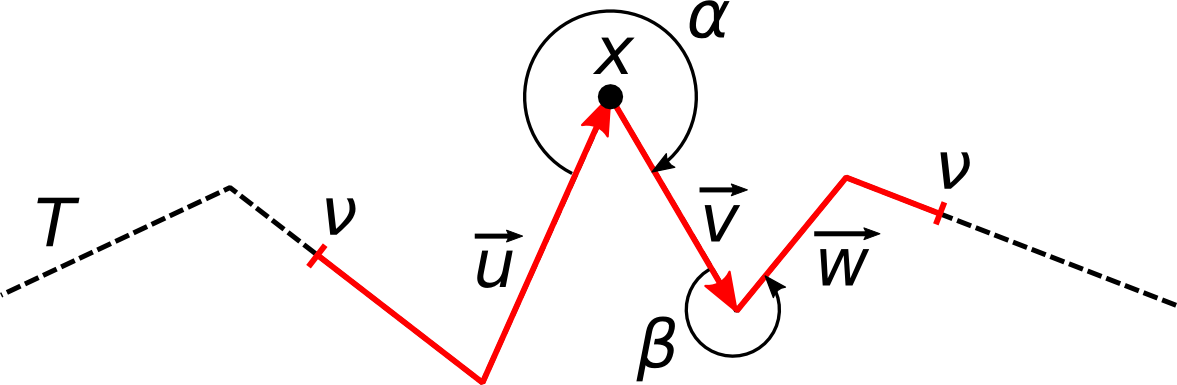
\includegraphics[width=0.95\linewidth]{img/complexity.png}
	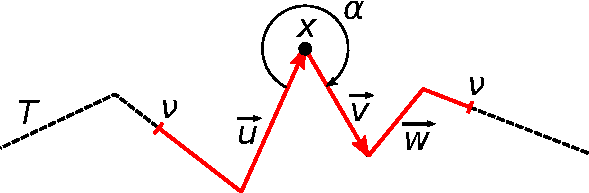
\includegraphics[width=0.95\linewidth]{img/complexity.pdf}
\caption{Evaluation of the complexity of a trajectory $T$ in point $x$.
The complexity $c(x)$ is determined by tuples $(u, v)$ and $(v, w)$, \ie their angles $\alpha$ and $\beta$, as the segments $u$, $v$, and $w$ lie in the neighborhood of $x$ (red).
The neighborhood of $x$ contains all points that are closer (along $T$) to $x$ than to $\nu$.}
\label{fig:complexity}
\end{figure}

Furthermore, the simplification $S$ is set to be empty at the beginning and the resulting trajectory $T_{out}$ is set to $T_{in}$.
The iterative simplification then proceeds as follows.
First, a set of simple points $P$ is found by thresholding $c(x)$ by $\tau$.
All points $p \in P$ are then removed from $C$ which prevents further simplification of parts of the trajectory that are already simple.
Then, $T_{out}$ is simplified in all complex intervals that remained in $C$.
After the simplification, the complexity is evaluated again and the improvement in comparison with the previous complexity is computed.
The iterative simplification ends when the improvement after an iteration $\Delta c$ drops below a user-specified threshold $\epsilon$.

To address the correctness issue, which may be raised by the smoothing simplification, we provide also non-smoothing simplification employing Douglas-Peucker algorithm~\cite{visvalingam1990douglas} which preserves original positions of trajectory vertices.
Generally, the non-smoothing simplification employs schemes presented in Algorithms~\ref{alg:simplify}~and~\ref{alg:auto-simplify}.
Only small modifications to the simplification data structure ($S$) and a new complexity measure $c_{DP}(x)$ were needed due to the nature of the Douglas-Peucker algorithm which keeps only a subset of its input positions.
We present only the new complexity measure since the other changes are trivial.
The complexity $c_{DP}(x)$ is defined as:
\begin{equation}
  c_{DP}(x) = \sum_{s \in N_{DP}(T, x, \nu)}{\frac{|s|}{|P_e - P_s|}},
\label{eq:complexity-dp}
\end{equation}
where $N_{DP}(T, x, \nu)$ is a set of trajectory segments in the neighborhood of $x$ (see Equation~\ref{eq:complexity}), and $P_s$ and $P_e$ are start and end points in that neighborhood.
Both simplification approaches were evaluated by the domain experts.
They concluded that, although the smoothing simplification is superior thanks to the ability to provide results that are easy to understand using visualization, it is also important for them to use the non-smoothing simplification to confirm their assumptions that were made when visualizing the smoothed variant.

\subsection*{Derivation of Attributes - JB}

In previous section we have described the simplification of the ligand trajectory. 
On one hand, such approximation helps to easily understand the overall ligand movements. 
On the other hand, it also suppresses vast amount of details that are important for the complete understanding of the ligand movements inside protein.

In order to preserve this information and hence allow the biochemist to explore the ligand behaviour in detail we evaluate various geometrical and chemico-physical attributes of the ligand trajectory on multiple levels. 
These attributes are then communicated to the user in various ways (for more details {\color{red}see Section~\ref{XYZ}}).

Among the most important attributes belongs the "stuckenss" of the ligand in one place, its distance from the active site, direction of its movement, amount of surrounding free space, changes of surrounding amino acids and its properties, and relative movements and rotations of the ligand inside the tunnel. 
In the rest of this section we discuss usefulness and the way how we derive individual attributes them from the original data.    

\begin{itemize}

\item \textbf{Stuckness} is one of the most abstract attributes. Fortunately, it can be easily measured. 
We consider the ligand to be stuck if it oscillates around specific place inside the protein tunnel (w.r.t. the active site). \todo{to w.r.t. musím doprogramovat - ale myslím, že to dáva smysl ne, počítat to vzheledem k AC??} 
In other words we need to evaluate the time for which the ligand remained on single spot. 
Since the original data are uniformly sampled (\eg we know exact ligand position every two femtoseconds), we can measure the distance between two subsequent time steps and immediately obtain the speed of the ligand movement in that particular area. 
The higher the speed of the ligand is, the higher distance it can travel and hence it is less stuck. \todo{nevím, zda stuck je to zprávné slovo}
The importance of the attribute follows from the fact that if the ligand gets stuck for some reason it will not proceed through the protein tunnel and hence it may not reach the active site quick enough for the desired reaction to happen.
Therefore the biochemists want to explore such cases in more detail in order to either evaluate the functionality of the protein or even change its properties by replacing some amino acids.


\item \textbf{Distance} of the ligand from the active site provide the biochemists with the information whether some observed behaviour occurred in vicinity of active site, surface, or somewhere along the path. 
This can be very helpful in cases when the biochemists, for instance, want to mutate (\ie change) some amino acids along the tunnel in order to lower the "stuckness" of the ligand in that area. 
In this case it is usefull to actually see where exactly the unwanted bahaviour of ligand is happening.
In order to evaluate the distance of the ligand from active site, we first extract the position of the active site in each time step. 
Note that the active site is denoted by set of surrounding amino acids. 
Hence, we can compute the position of the active site as the center of mass of these amino acids. 
Once we have the position of active site, we simply measure its distance from the center of mass of ligand atoms.
      
\item \textbf{Direction} of the ligand movement w.r.t. the active site is another very important attribute. 
During the molecular dynamics simulation the ligand can enter and again leave the protein tunnel multiple times. 
Therefore, the biochemists are interested in distinguishing between intervals where the ligand was traveling towards the active site and where it was traveling in the opposite side (\ie towards the outer environment). 
In order to obtains this information we first compute the distance between active site and ligand (computed in aforementioned way) in each time step. 
Afterwards, we evaluate weather this distance is decreasing in two subsequent time steps -- in such case we consider the ligand to be moving towards the active site. 
Similarly, if the distance is getting higher we mark the ligand to be moving towards the protein surface.        

\item \textbf{Amount of free space} surrounding the ligand can help the biochemists to evaluate one of the reasons behind the lingad beeing stuck. 
It was shows in many studies {\color{red}\eg cite some caver?} that the geometrical properties (\eg width) of the protein tunnel play a crucial role when determining reactivity between proteins and ligands. 
In our case the low width of the tunnel may prevent the ligand from progressing through the tunnel and hence explain cases when the "stuckness" attribute is high. 
In order to evaluate free space surrounding the ligand we used the temporal tunnel (see Section~\ref{Sec:TemporalTunnel}\todo{bez cisel se neda odkazovat na sekce!!!}). 
The definition of temporal tunnel ensures that each its sphere corresponds exactly to a single time step and the ligand lies inside it. 
Since each such sphere also corresponds to the empty space in that part of protein in given time step, we can directly use its radius to define this "amount of free space" attribute. \todo{ta poslední věta je na dvě věci, ale nenapadá mě jak jinak}

\item \textbf{Changes of amino acids and its properties} is another very important aspect of ligand trajectory evaluation.
First, the changes of amino acids can show the parts of the trajectory where the ligand  significantly changed its position w.r.t. the molecule itself. 
The higher number of different amino acids surrounding the ligand between two time steps means the higher shift inside the protein tunnel.
Moreover, whether the ligand will be able to pass through the tunnel and reach the active site, is highly depended not only on geometric properties of the tunnel but also on its physico-chemical properties (\eg hydrophobicity or electric charge).
\todo{tady to bude chtít nějak lépe napojit}The individual biochemical properties are determined by surrounding amino acids.
It might be usefull for biochemists to observe such physico-chemical properties and hence evaluate its influence on the ligand stuckness. \todo{pokud by jste chtěli, je možno tu dopsat, že hydrophobicita je průměr okolí, el. charge bude normálně podle zákona o sčítání potenionálu, atd.} 

{\color{red}\item \textbf{Relative movements and rotations} of ligands není implementováno, takže se nebudu párat zatím s tím, abych to tu popisoval, když ani zatím nevím, jak to implementovat} 

\item \textbf{Straightness} \todo{Adame?}

\end{itemize}


time evolution, "stuckness" (speed, distance), direction, amount of free space around (radius), AA changes + properties, vorticity, ligand deformation (dihedral angles)

\section*{Visual Exploration}

\subsection*{Data Views - BK + ladies}
motivation, design

3D, bar charts, scatterplot

\subsubsection*{3D View}

\subsubsection*{Barchart View}


The information about the surrounding acids is also very crucial when exploring the ligand bottlenecks. 
For each time step within the temporal block we compute the three closest amino acids from the ligand. 
We provide the visual representation of this list (Fig.~\ref{fig:aacids}), where each amino acid defines one line in the list. 
The line is colored with respect to a selected physico-chemical property~---~our representation supports switching between hydrophobicity, partial charges, and donors and acceptors.
The interruption in some of these lines is caused by the fact that the given amino acid is not present around the ligand in the corresponding temporal block.

\begin{figure}[htb]
	\centering
  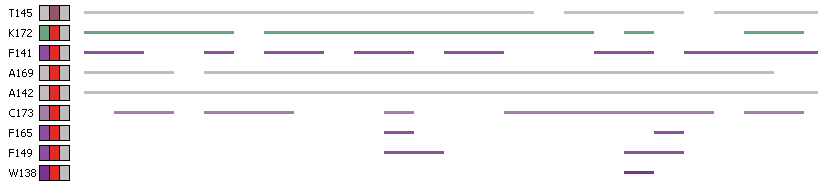
\includegraphics[width=0.95\linewidth]{img/aacids.png}
  \caption{\label{fig:aacids} Representation of amino acids surrounding the temporal tunnel and their physico-chemical properties. Coloring corresponds to a selected property, the line interruption means that this amino acid was not detected around the ligand in the corresponding temporal block.}
\end{figure}


\subsubsection*{Scatterplot Matrix}
For detailed analysis of geometrical and chemico-physical attributes of the ligand trajectory at given time steps, we propose Scatterplot Matrix.
The axes of one scatterplot represent a pair user-selected attributes.
Each point in the scatterplot then represents the values of these attributes at one time step.
As a result the scatterplot can easily reveal trends and relationships between attributes.
Interactive manipulation with scatterplot, such as selection, zooming and change of displayed attributes provides easy way of manual data filtering. 
To eliminate the noise in the data caused by ligand jittering, we propose several smoothing and aggregation functions.
\todo{nechat len sliding window?} 
The Sliding Window function assigns to each time step averaged value of its neighborhood.
The size of the neighborhood is user regulated. 

The plots can further be stacked, forming a matrix and thus showing relationship between multiple attributes at once.
The stacked plots are also interactively interconnected.
The selection in Scatterplot Matrix is interactively linked with Barchart View.

Figure \ref{fig:scatterplot} shows Scatterplot Matrix for a sequence of $500$ time steps.

\begin{figure}[htb]
	\centering
  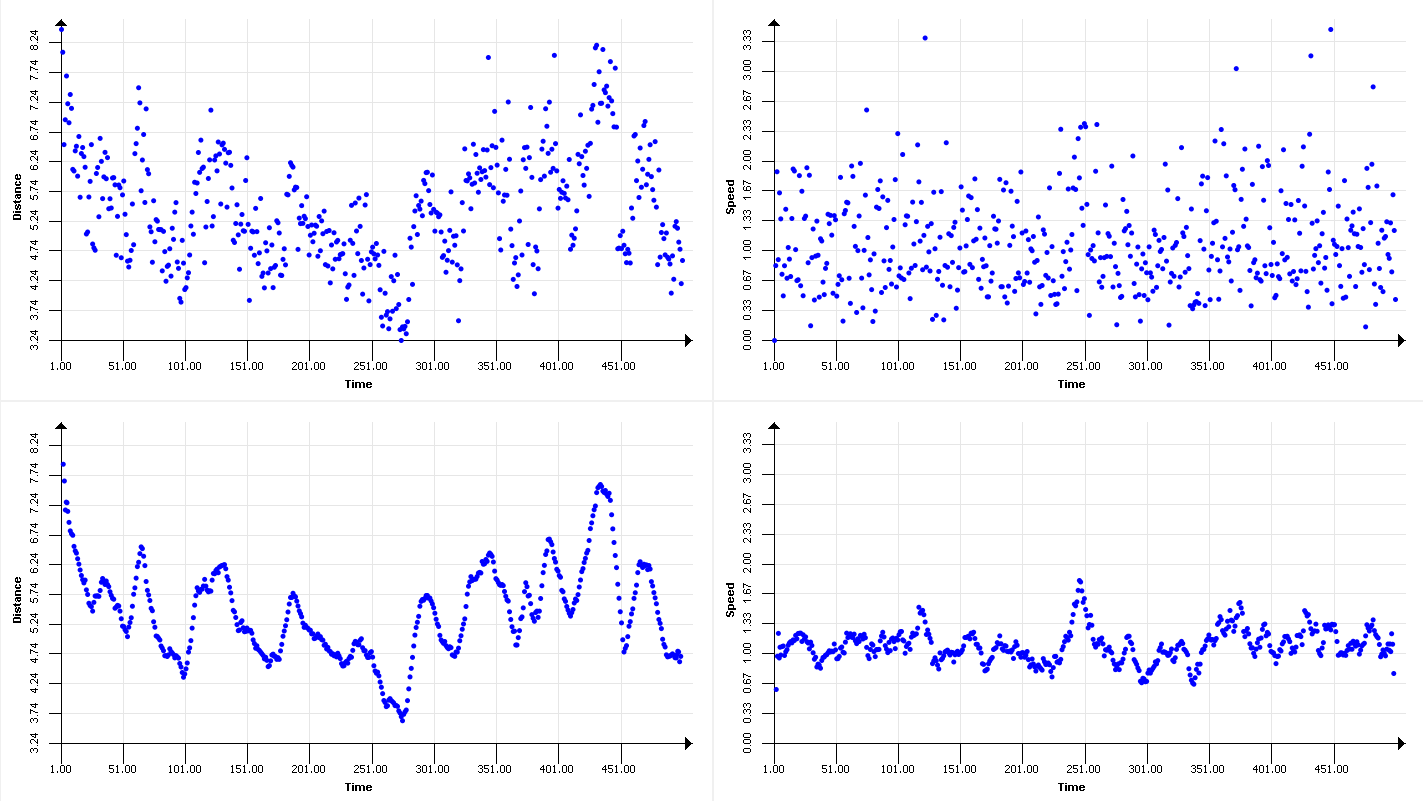
\includegraphics[width=0.95\linewidth]{img/scatterplot.png}
  \caption{\label{fig:scatterplot} CHANGE!!! Scatterplot Matrix depicting Time vs. Distance and Time vs Speed property before (up) and after (down) smoothing by Sliding Window function.}
\end{figure}


\subsection*{Analysis Procedure - BK, JP, JB}
In this section we will describe one of case studies which we have performed using our novel exploration tool.
In this particular study biochemists explored molecular simulation of Haloalkane dehalogenase protein together with its ligand. 
Since the simulation consists of 50000 snapshots, it would take an enormous amount of time to analyze it using only common techniques such as 3D animation.
In this section we will show how this can be significantly improved using our exploration tool.
After the precomputation stage the user can start to explore individual views described in previous sections.

We start with the rough analysis of the overall behavior of the ligand using our simulation overview (see Figure \ref{fig:case_overview}).

\begin{figure}[htb]
	\centering
  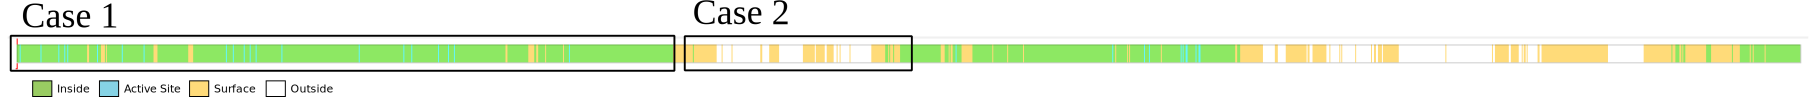
\includegraphics[width=0.95\linewidth]{img/case_overview.png}
  \caption{\label{fig:case_overview} {\color{red}TODO}}
\end{figure}

Utilizing this view the biochemist can immediately see that the whole simulation consist basically from two parts (divided by yellow color signalizing that tunnel was moving near the protein surface).

{\color{red} když na to tak koukám, tak mám pocit, že ten overview je tak trošku na ....dvě věci, asi to krapet předělám....}







\section*{Results and Discussion - BK}
use case + feedback

\section*{Conclusions - All}
and future work 

%%%%%%%%%%%%%%%%%%%%%%%%%%%%%%%%%%%%%%%%%%%%%% 
%%                                          %%
%% Backmatter begins here                   %%
%%                                          %%
%%%%%%%%%%%%%%%%%%%%%%%%%%%%%%%%%%%%%%%%%%%%%%

\begin{backmatter}

\section*{Competing interests}
The authors declare that they have no competing interests.


%%%%%%%%%%%%%%%%%%%%%%%%%%%%%%%%%%%%%%%%%%%%%%%%%%%%%%%%%%%%%
%%                  The Bibliography                       %%
%%                                                         %%
%%  Bmc_mathpys.bst  will be used to                       %%
%%  create a .BBL file for submission.                     %%
%%  After submission of the .TEX file,                     %%
%%  you will be prompted to submit your .BBL file.         %%
%%                                                         %%
%%                                                         %%
%%  Note that the displayed Bibliography will not          %%
%%  necessarily be rendered by Latex exactly as specified  %%
%%  in the online Instructions for Authors.                %%
%%                                                         %%
%%%%%%%%%%%%%%%%%%%%%%%%%%%%%%%%%%%%%%%%%%%%%%%%%%%%%%%%%%%%%

% if your bibliography is in bibtex format, use those commands:
\bibliographystyle{bmc-mathphys} % Style BST file
\bibliography{bmc_article}      % Bibliography file (usually '*.bib' )

% or include bibliography directly:
% \begin{thebibliography}
% \bibitem{b1}
% \end{thebibliography}

%%%%%%%%%%%%%%%%%%%%%%%%%%%%%%%%%%%
%%                               %%
%% Figures                       %%
%%                               %%
%% NB: this is for captions and  %%
%% Titles. All graphics must be  %%
%% submitted separately and NOT  %%
%% included in the Tex document  %%
%%                               %%
%%%%%%%%%%%%%%%%%%%%%%%%%%%%%%%%%%%

%%
%% Do not use \listoffigures as most will included as separate files

%\section*{Figures}
%  \begin{figure}[h!]
 % \caption{\csentence{Sample figure title.}
  %    A short description of the figure content
   %   should go here.}
   %   \end{figure}

%\begin{figure}[h!]
 % \caption{\csentence{Sample figure title.}
  %    Figure legend text.}
  %    \end{figure}

%%%%%%%%%%%%%%%%%%%%%%%%%%%%%%%%%%%
%%                               %%
%% Tables                        %%
%%                               %%
%%%%%%%%%%%%%%%%%%%%%%%%%%%%%%%%%%%

%% Use of \listoftables is discouraged.
%%
%\section*{Tables}
%\begin{table}[h!]
%\caption{Sample table title. This is where the description of the table should go.}
 %     \begin{tabular}{cccc}
%        \hline
 %          & B1  &B2   & B3\\ \hline
 %       A1 & 0.1 & 0.2 & 0.3\\
 %       A2 & ... & ..  & .\\
 %       A3 & ..  & .   & .\\ \hline
 %     \end{tabular}
%\end{table}

%%%%%%%%%%%%%%%%%%%%%%%%%%%%%%%%%%%
%%                               %%
%% Additional Files              %%
%%                               %%
%%%%%%%%%%%%%%%%%%%%%%%%%%%%%%%%%%%

%\section*{Additional Files}
%  \subsection*{Additional file 1 --- Sample additional file title}
%    Additional file descriptions text (including details of how to
%    view the file, if it is in a non-standard format or the file extension).  This might
%    refer to a multi-page table or a figure.

%  \subsection*{Additional file 2 --- Sample additional file title}
%    Additional file descriptions text.

\end{backmatter}
\end{document}
